\documentclass{beamer}

\usetheme[]{Rochester}
\usecolortheme{beaver}
\usepackage[latin1]{inputenc}
\usepackage{graphics}

\author{Will Webberley}
\date{Autumn 2014}
\institute[COMSC]{Cardiff School of Computer Science and Informatics}



\title{The `Physical' Interface: Hardware}
\subtitle{CM2101: Human-Computer Interaction}

\begin{document}

\frame{\titlepage}

\frame{
    \frametitle{Hardware interface}
    \begin{itemize}
        \item The direct link between a human and an electronic system
        \item Forms a layer of abstraction between the user's cognitive model and the system model
        \item Part of the gulfs of execution and evaluation
        \item Used for input (\alert{execution}) and output (\alert{evaluation})
        \item For manipulating, pointing, knowledge transfer, guiding, etc.
    \end{itemize}
}

\frame{
    \frametitle{Hardware interface for humans}
    \begin{center}
        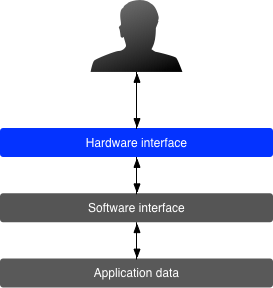
\includegraphics[width=6cm]{media/hardware_interface.png}
    \end{center}
}

\frame{
    \frametitle{Hardware interface}
    \begin{itemize}
        \item Can also be a link between the \alert{environment} and a system
        \item Useful to know some of the things that can be detected 
        \item An automatic \alert{input} from the environment may provide \alert{output} for a user
        \begin{itemize}
            \item In many phones, if environment is brighter, the screen backlight automatically brightens
        \end{itemize}
   \end{itemize}
}

\frame{
    \frametitle{Environmental inputs}
    The following can be detected by hardware for (automatically) informing systems and users:
    \begin{itemize}
        \item Temperature (environmental systems - e.g. for meteorology)
        \item Air quality (smoke alarms - e.g. \alert{Nest})
        \item Sound 
        \item Electromagnetic spectrum (e.g. `light' for automatic street lamps, `infrared' for surveillance, `radio' for communication)
        \item Movement (accelerometry)
        \item Magnetic fields (e.g. compasses)
    \end{itemize}
    \vskip10pt
    Most of these exist in everyday devices, including many smartphones
}


\frame{
    \frametitle{Hardware interfaces in user evaluation}
    \begin{itemize}
        \item Users need to use the interface in order to use the system
        \item Hardware interface may help or hinder user
        \item By changing the hardware interface, can we:
        \begin{itemize}
            \item Help address some usability principles (for example, \alert{Satisfaction} or \alert{Learnability})
            \item Hardware interface might be inappropriate for users of the system
        \end{itemize}
    \end{itemize}
}

\frame{
    \frametitle{Hardware interfaces in cognitive modelling}
    \begin{itemize}
        \item \alert{Operators} stage of GOMS related to the hardware interface
        \item e.g. pressing buttons, tapping screen, clicking mouse
        \item KLM measures the time taken to complete a task from sum of physical operators
        \item By changing the hardware interface, can we reduce:
        \begin{itemize}
            \item Cognitive burden of the system's users
            \item Time taken to complete the system's tasks
        \end{itemize}
    \end{itemize}
}

\frame{
    \frametitle{Using multiple input interfaces}
    \begin{itemize}
        \item Some systems may use multiple interfaces for the same task
        \item For example, Android keyboard
        \begin{itemize}
            \item Supports key-presses or swiping (touchscreen interaction)
            \item Supports voice-input (voice interaction)
        \end{itemize}
    \end{itemize}
}

\frame{
    \frametitle{Using multiple output interfaces}
    \begin{itemize}
        \item Systems use multiple output interfaces to provide richer functionality
        \item For example, most modern games 
        \begin{itemize}
            \item \alert{Visual} - graphics, imagery
            \item \alert{Audio} - sounds, music
            \item \alert{Tactile} - haptic feedback (console controllers, mobile devices)
        \end{itemize}
    \end{itemize}
}

\frame{
    \frametitle{Output devices}
    \begin{itemize}
        \item Peripheral hardware
        \item To inform the user (or other systems) about information
        \item Conveys the result of data processing
        \item Usually convert low-level electronic information into a human-understandable form
    \end{itemize}
}

\frame{
    \frametitle{Output devices: examples}
    \alert{Display devices}
    \begin{columns}
        \column{.7\textwidth}
            \begin{itemize}
                \item Types
                \begin{itemize}
                    \item LCD, (AMO)LED, plasma, CRT, projection, etc. (e.g. displays, TVs)
                    \item Lower quality LCD (e.g. calculators, alarm clocks)    
                \end{itemize}
                \item Uses
                \begin{itemize}
                    \item Displaying text (e.g. consoles)
                    \item Displaying graphics (e.g. GUIs - need some kind of graphics processing hardware)
                    \begin{itemize}
                        \item For images, movies, games, etc.
                    \end{itemize}
                    \item Notifications
                \end{itemize}
            \end{itemize}
        \column{.3\textwidth}
            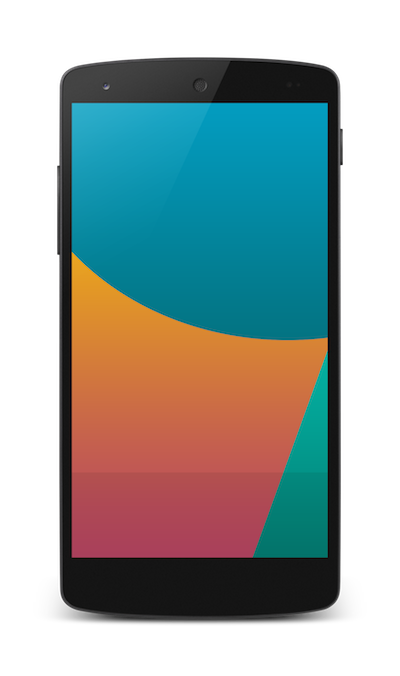
\includegraphics[width=4cm]{media/nexus_5.png}
    \end{columns}
}

\frame{
    \frametitle{Output devices: examples}
    \alert{Audio devices}
    \begin{columns}
        \column{.7\textwidth}
            \begin{itemize}
                \item Types
                \begin{itemize}
                    \item Speakers, head/earphones (high-fidelity audio)
                    \item Beepers (low-fidelity audio)
                \end{itemize}
                \item Uses
                \begin{itemize}
                    \item Voice output (e.g. navigation, hands-free, telephone/VOIP)
                    \item Sound output (e.g. music or entertainment)
                    \item Notification (e.g. smartphone alerts)
                    \item Feedback (e.g. in games, keyboard-presses)
                \end{itemize}
            \end{itemize}
        \column{.3\textwidth}
            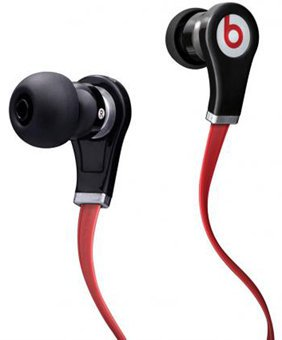
\includegraphics[width=3cm]{media/beats.jpg}
    \end{columns}
}

\frame{
    \frametitle{Output devices: examples}
    \alert{Tactile devices}
    \begin{columns}
        \column{.7\textwidth}
            \begin{itemize}
                \item Types
                \begin{itemize}
                    \item Haptics (e.g. applying forces, vibrations, motions to user)
                \end{itemize}
                \item Uses
                \begin{itemize}
                    \item Feedback (e.g. in games)
                    \item Notification (e.g. smartophone alerts)
                \end{itemize}
            \end{itemize}    
        \column{.3\textwidth}
            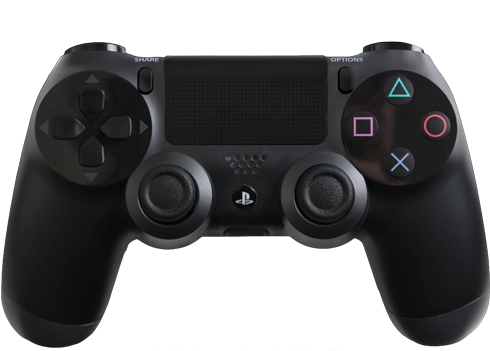
\includegraphics[width=3cm]{media/ps4_controller.png}
    \end{columns}   
}

\frame{
    \frametitle{Output devices: examples}
    \alert{Printing devices}
    \begin{columns}
        \column{.7\textwidth}
            \begin{itemize}
                \item Types
                \begin{itemize}
                    \item Paper printer (e.g. for documents, photos)
                    \item Embosser (e.g. in braille-printers)
                    \item 3D printer (e.g. for low-cost object manufacture)
                \end{itemize}
                \item Uses
                \begin{itemize}
                    \item `Soft' to `hard' material
                    \item Reporting and reading
                    \item Enhancing the physical world
                \end{itemize}
            \end{itemize}    
        \column{.3\textwidth}
            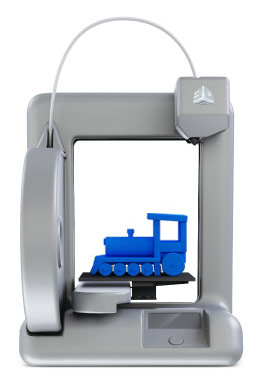
\includegraphics[width=4cm]{media/cube.jpg}
    \end{columns}   
}

\frame{
    \frametitle{Output devices: examples}
    \alert{Visible light devices}
    \begin{columns}
        \column{.7\textwidth}
            \begin{itemize}
                \item Types
                \begin{itemize}
                    \item LED (e.g. in electronics)
                    \item Bulb (for brighter use)
                \end{itemize}
                \item Uses
                \begin{itemize}
                    \item Indicating status (e.g. red vs. green LEDs on electronics)
                    \item Instruction or warning (e.g. traffic lights)
                    \item Entertainment (light shows, clubs, etc.)
                \end{itemize}
            \end{itemize}    
        \column{.3\textwidth}
            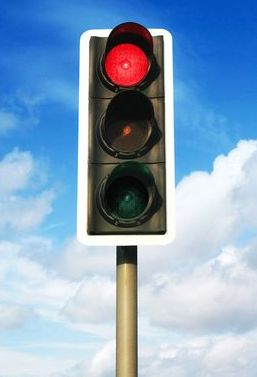
\includegraphics[width=3cm]{media/traffic_light.jpg}
    \end{columns}   
}

\frame{
    \frametitle{Output devices: examples}
    \alert{Electromagnetic transmission devices}
    \begin{columns}
        \column{.7\textwidth}
            \begin{itemize}
                \item Types
                \begin{itemize}
                    \item Radio transmitters 
                    \item Infrared transmitters 
                \end{itemize}
                \item Uses
                \begin{itemize}
                    \item \textbf{Machine-machine communication}
                    \item Remote controls
                    \item TV and radio broadcast 
                    \item Cellular network communication, WiFi, BlueTooth
                \end{itemize}
            \end{itemize}    
        \column{.3\textwidth}
            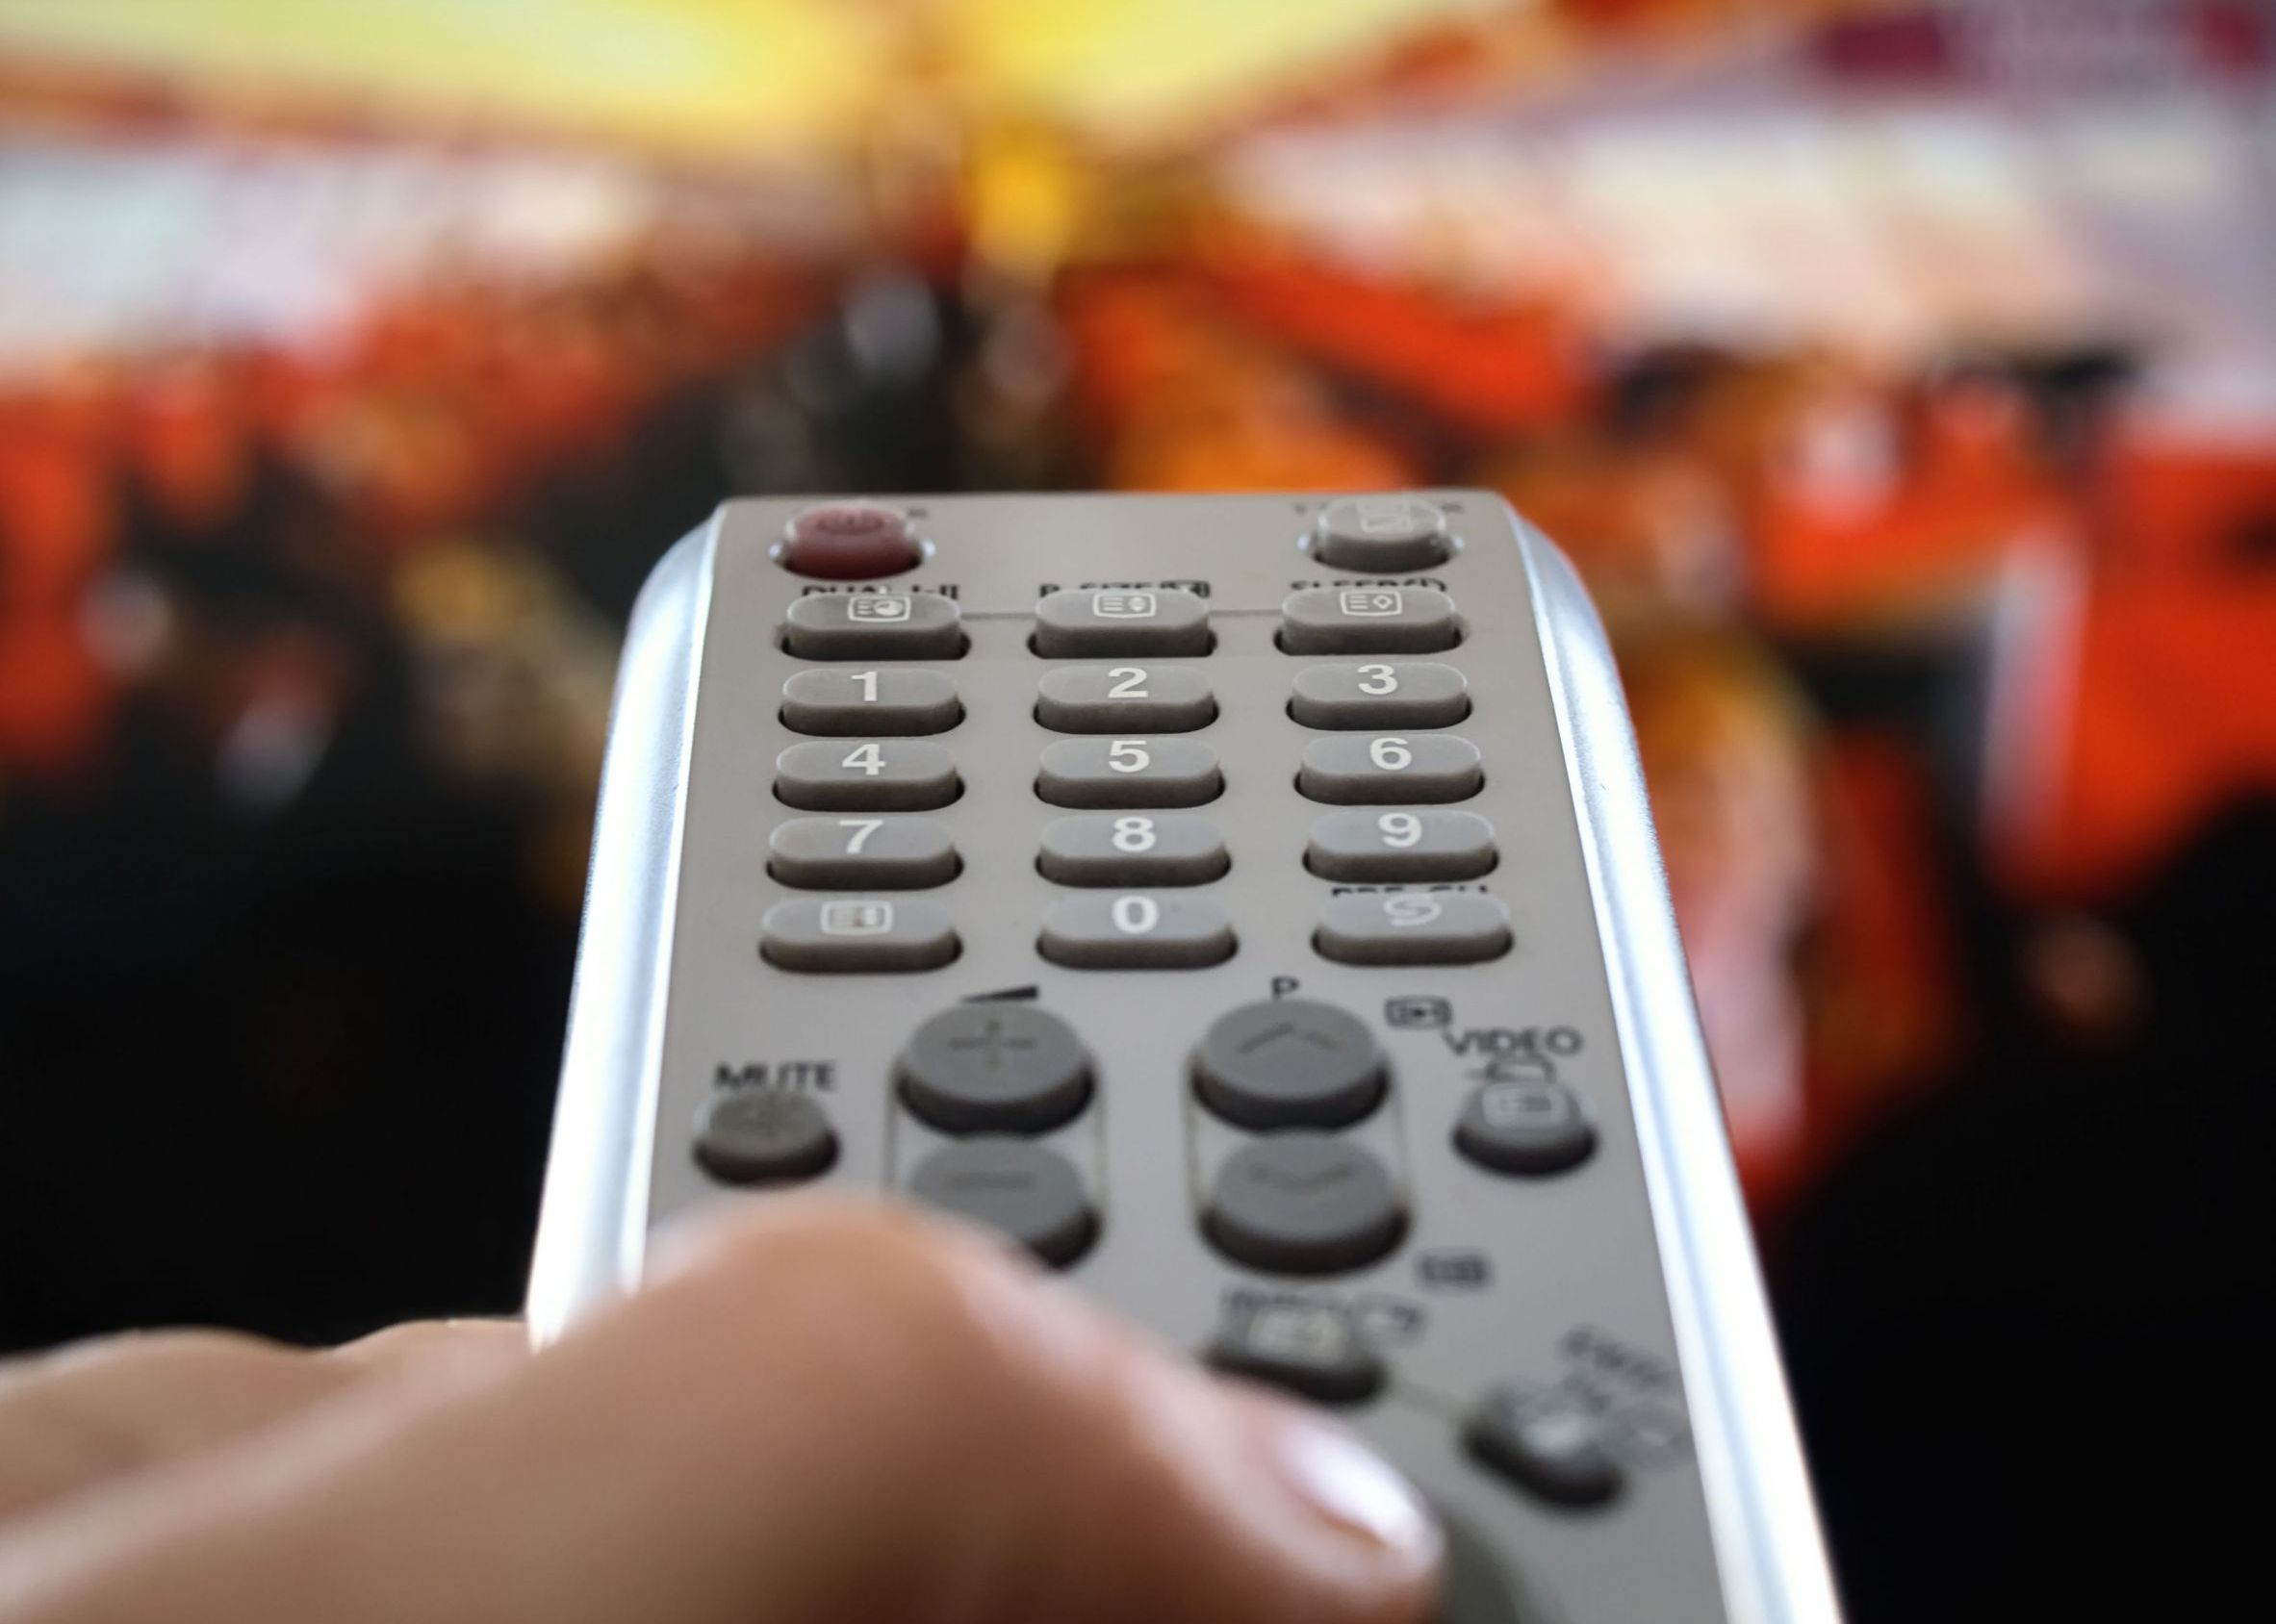
\includegraphics[width=3cm]{media/remote_control.jpg}
    \end{columns}   
}

\frame{
    \frametitle{Input devices}
    \begin{itemize}
        \item Peripheral hardware
        \item To inform the system about some information    
        \item To provide data to be processed
        \item Converts human (or environmental) `knowledge' into low-level electronic information
    \end{itemize}
}

\frame{
    \frametitle{Input devices: examples}
    \alert{Pointer devices}
    \begin{columns}
        \column{.5\textwidth}
            \begin{itemize}
                \item Types
                \begin{itemize}
                    \item Mouse (multi-button)
                    \item Trackpad
                    \item Rollerball
                \end{itemize}
                \item Uses
                \begin{itemize}
                    \item Moving cursors
                    \item Providing direction
                    \item Navigation
                    \item Games
                \end{itemize}
            \end{itemize}    
        \column{.5\textwidth}
            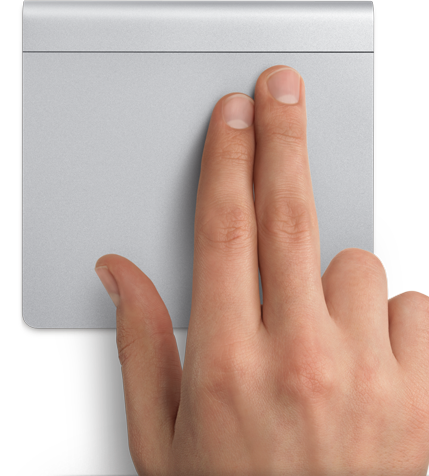
\includegraphics[width=4cm]{media/trackpad.png}
    \end{columns}   
}

\frame{
    \frametitle{Input devices: examples}
    \alert{Keyboard devices}
    \begin{columns}
        \column{.7\textwidth}
            \begin{itemize}
                \item Types 
                \begin{itemize}
                    \item Keyboard (e.g. for computers)
                    \item Keypad (e.g. for phones)
                \end{itemize}
                \item Uses
                \begin{itemize}
                    \item `Formal' data input (text, numbers, etc.)
                    \item Navigation
                    \item Games
                \end{itemize}
            \end{itemize}    
        \column{.3\textwidth}
            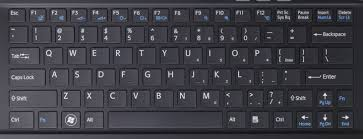
\includegraphics[width=3cm,angle=30]{media/keyboard.jpg}
    \end{columns}   
}

\frame{
    \frametitle{Input devices: examples}
    \alert{Imaging devices}
    \begin{columns}
        \column{.7\textwidth}
            \begin{itemize}
                \item Types 
                \begin{itemize}
                    \item Cameras (webcams, cameras)
                    \item Composite sensors (e.g. Kinect)
                    \item Document/image canners
                    \item Specialised (retina scanner, fingerprint scanner, barcode scanner, 3D scanner)
                    \item Medical (e.g. MRI)
                \end{itemize}
                \item Uses
                \begin{itemize}
                    \item Replication (printed images, objects)
                    \item Recording (movies, CCTV)
                    \item Less `formal' data entry (e.g. scanning barcodes)
                \end{itemize}
            \end{itemize}    
        \column{.3\textwidth}
            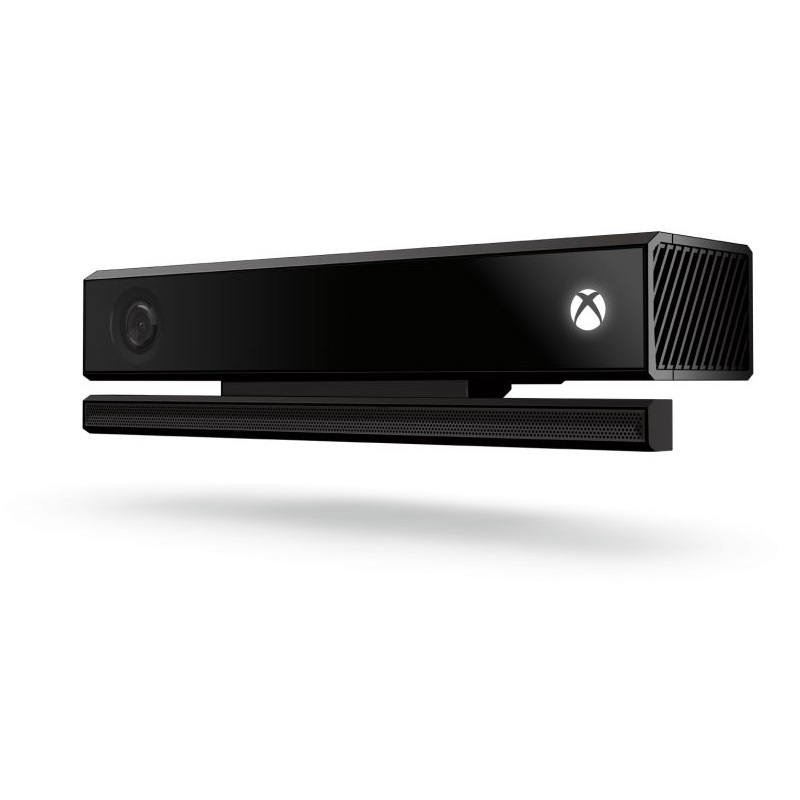
\includegraphics[width=4cm]{media/kinect.jpg}
    \end{columns}   
}

\frame{
    \frametitle{Input devices: examples}
    \begin{columns}
        \column{.6\textwidth}
            \alert{Audio input devices}
            \begin{itemize}
                \item Types 
                \begin{itemize}
                    \item Microphone
                \end{itemize}
                \item Uses
                \begin{itemize}
                    \item `Text' entry (for voice keyboards)
                    \item Virtual assistants (for Google Now, Siri)
                    \item Recording voice or sound (for entertainment)  
                    \item Voice or sound recognition (e.g. for Shazam, voice detection)
                \end{itemize}
            \end{itemize}    
        \column{.4\textwidth}
            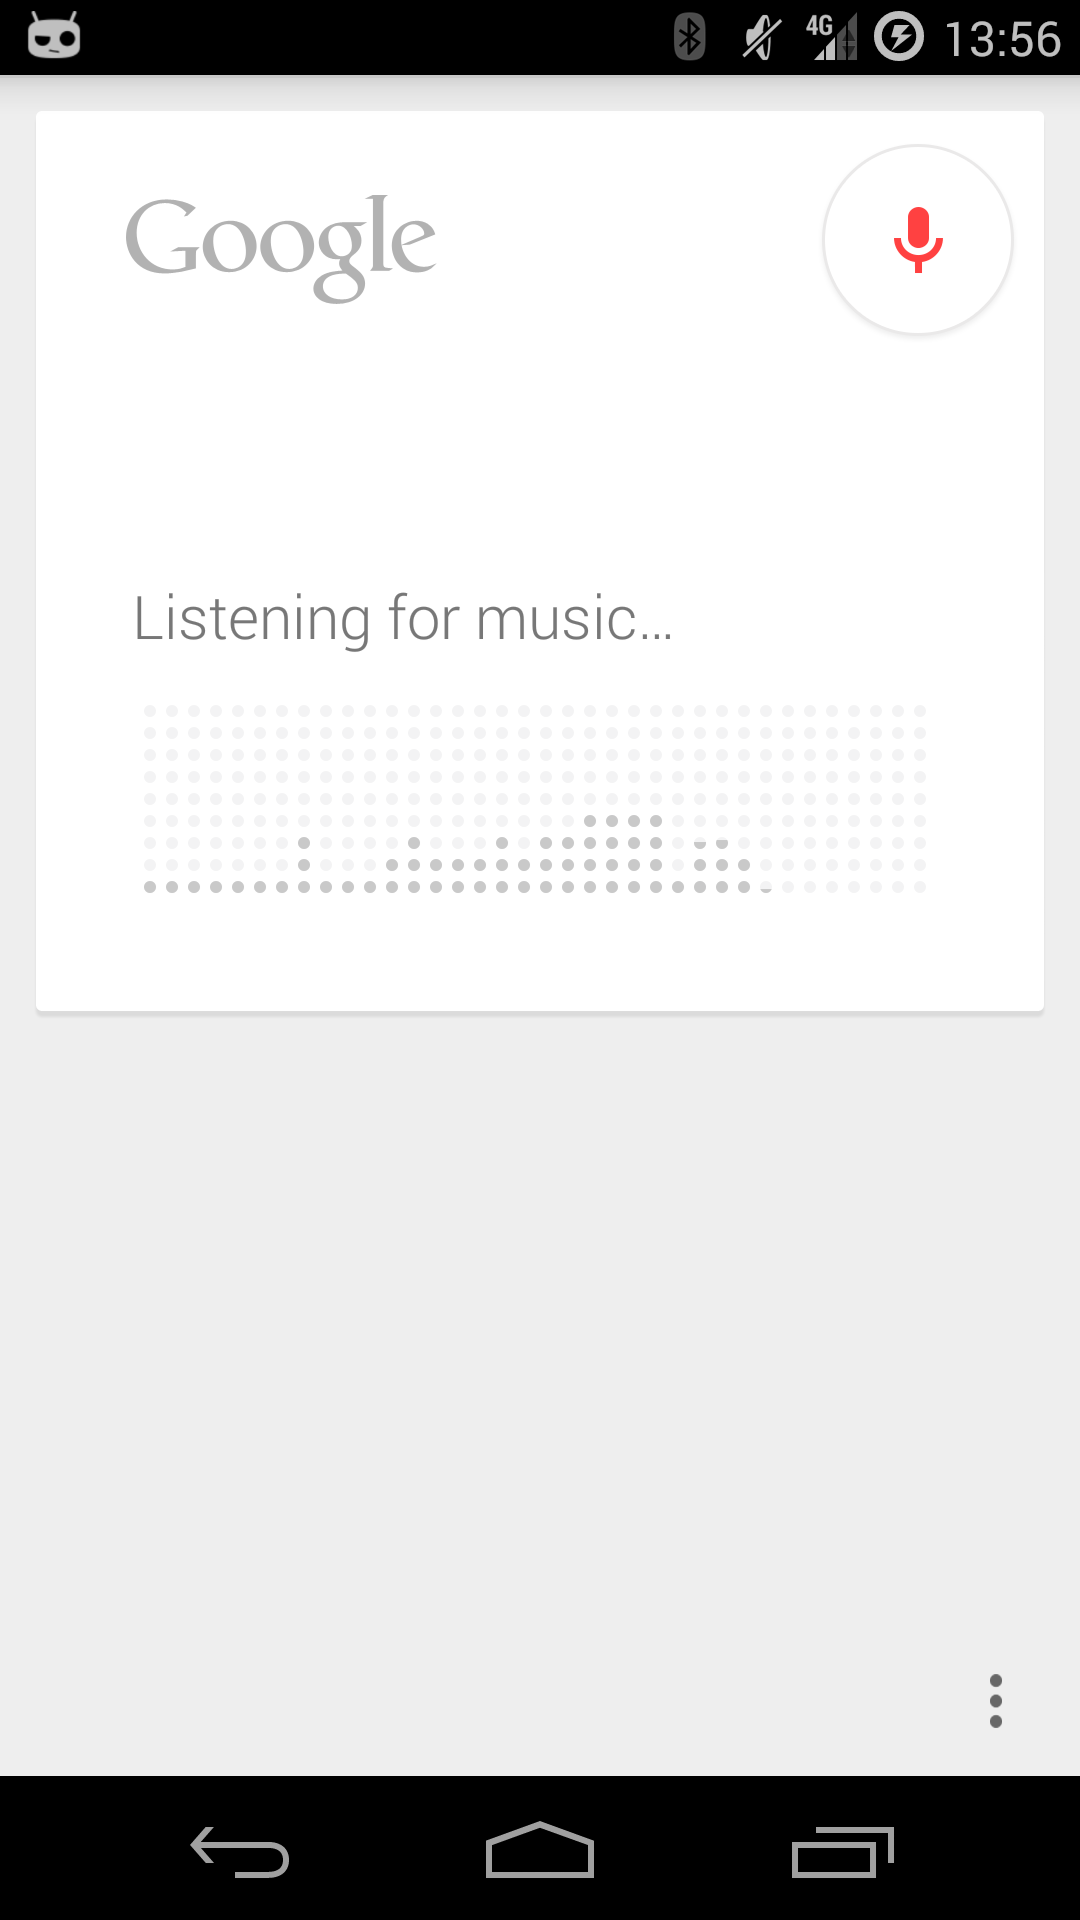
\includegraphics[width=4cm]{media/music_listen.png}
    \end{columns}   
}

\frame{
    \frametitle{Input devices: examples}
    \begin{columns}
        \column{.6\textwidth}
            \alert{Tactile input devices}
            \begin{itemize}
                \item Types 
                \begin{itemize}
                    \item Accelerometer
                \end{itemize}
                \item Uses
                \begin{itemize}
                    \item Navigation
                    \item Game control
                    \item Screen orientation control
                    \item Automatic image levelling
                    \item Automatic video stabalising 
                \end{itemize}
            \end{itemize}    
        \column{.4\textwidth}
            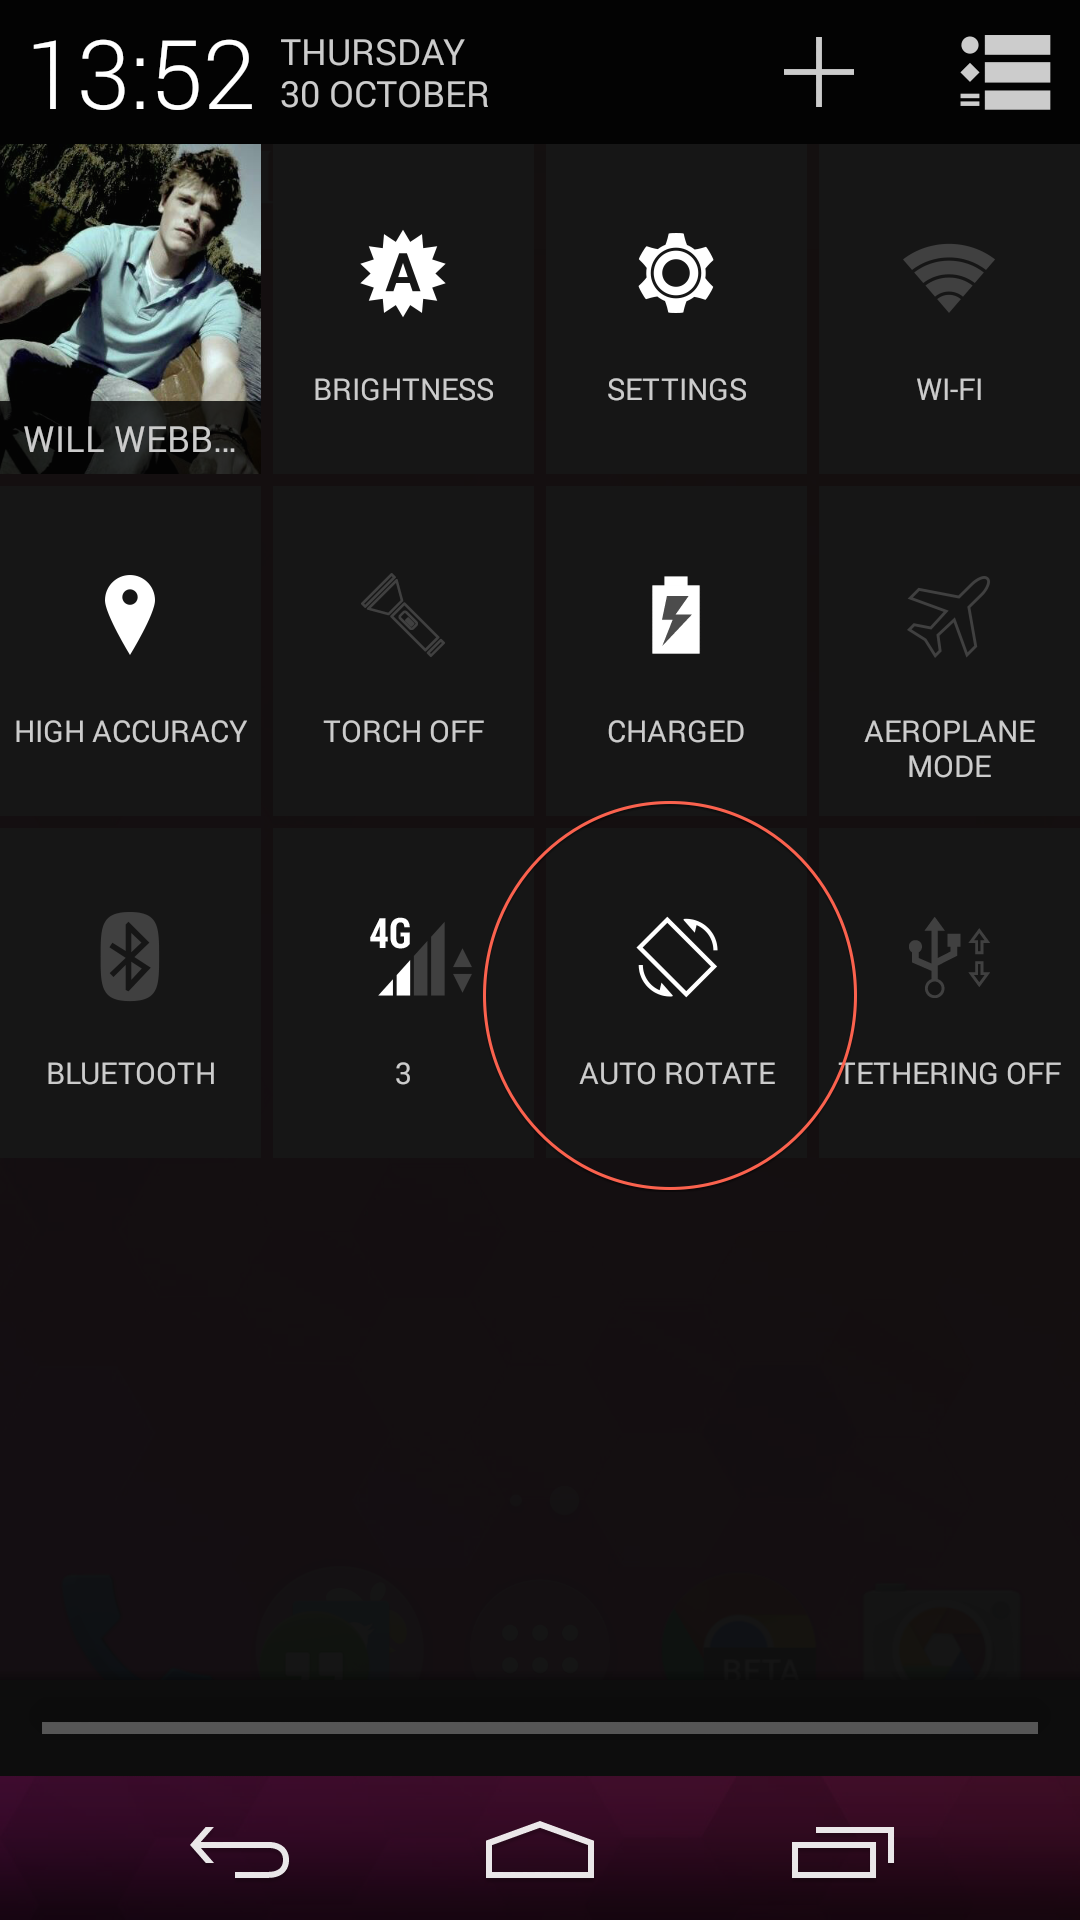
\includegraphics[width=4cm]{media/auto_rotate.png}
    \end{columns}   
}

\frame{
    \frametitle{Input devices: examples}
    \begin{columns}
        \column{.6\textwidth}
            \alert{Composite input devices}
            \begin{itemize}
                \item Types (typiclly > 2 types of input)
                \begin{itemize}
                    \item Gamepad
                    \item Wii Remote 
                \end{itemize}
                \item Uses
                \begin{itemize}
                    \item Navigation
                    \item Game control
                \end{itemize}
            \end{itemize}    
        \column{.4\textwidth}
            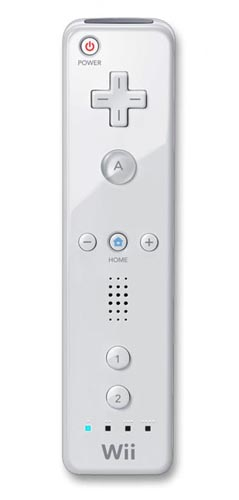
\includegraphics[width=3cm]{media/wiimote.jpg}
    \end{columns}   
}

\frame{
    \frametitle{Input devices: examples}
    \begin{columns}
        \column{.5\textwidth}
            \alert{Touchscreens}
            \begin{itemize}
                \item Types
                \begin{itemize}
                    \item Resistive (e.g. with stylus)
                    \item Capacitive (`touch-sensitive') 
                \end{itemize}
                \item Uses
                \begin{itemize}
                    \item Input for mobile devices
                    \item Multi-touch gesturing
                \end{itemize}
            \end{itemize}    
        \column{.5\textwidth}
            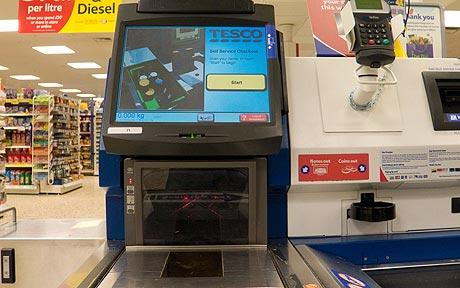
\includegraphics[width=5cm]{media/checkout.jpg}
    \end{columns}   
}

\frame{
    \frametitle{Input devices: examples}
    \alert{Many more}
    \begin{columns}
        \column{.5\textwidth}
            \begin{itemize}
                \item Buttons (binary: on or off)
                \item Switches (binary)
                \item Levers (binary)
                \item Dials (analogue)
                \item Pedals (analogue)
                \item Joystick (analogue / binary)
                \item ...
            \end{itemize}
        \column{.5\textwidth}
            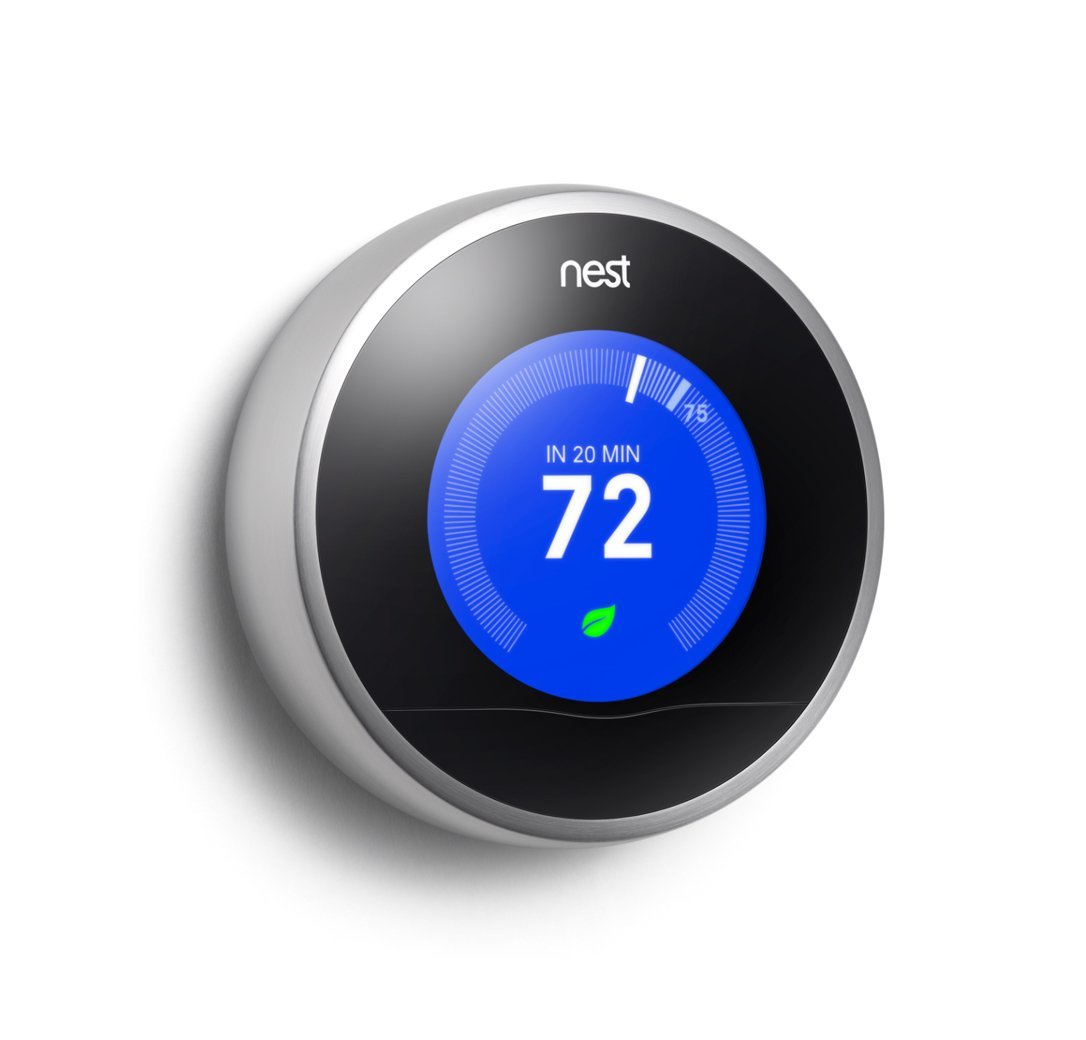
\includegraphics[width=5cm]{media/thermostat.jpg}
    \end{columns}
}

\frame{
    \frametitle{Hardware in general}
    \begin{itemize}
        \item Most systems need hardware to support both input and output
        \item This can be the \alert{same interface} (e.g. touchscreen)
        \item Most systems feature many hardware interfaces
        \item Many systems require a hardware interface to control a software interface...
        \item ... though not always the case (e.g. voice-text input)
    \end{itemize}    
}

\frame{
     \frametitle{Revision questions}
     \begin{enumerate}
        \item How does the hardware interface help bridge the gulfs of execution and evaluation?
        \item Name four environmental features detectable by standard hardware. How are these useful?
        \item What is the relevance of hardware in cognitive modelling?
        \item In what circumstances might hardware hinder the user of a system?
        \item Give an example of a system that uses multiple hardware interfaces for input and output.
        \item What is the point of a hardware output device? Give three examples of such a device.
        \item Give three examples of hardware input devices. What kind of data to they input?
        \item Explain and give an example of a single hardware interface supporting both input and output.
     \end{enumerate}
}

\frame{
    \frametitle{Summary}
    \begin{itemize}
        \item Use of hardware interfaces in interactive systems
        \item Evaluation (user+cognitive) of hardware devices in systems
        \item Use of multiple hardware devices
        \item Environment-machine, human-machine, machine-machine input/output
        \item Output hardware devices
        \item Input hardware devices
    \end{itemize}
}    

\end{document}
